\section{Results}\label{sec:results}

\subsection{($\lambda, \lambda$) scheme}


The Friedman Test showed significant difference in values among tournament size values across all functions, for any configuration, with the uniform crossover. This results hold for every scenario with 10, 20, and 40 dimensions, given: all functions (unimodal or multimodal); or only the multimodal functions. There is except when considering the results with the uniform crossover, for the unimodal group of functions. Also, for group of all function with 40 dimensions and the uniform crossover, there was found no significant difference in the results. The results can be better analyzed in the following Tables~\ref{Friedman_test_uniformed}, ~\ref{Friedman_test_sbx}.


\begin{table}[h]
	\centering
	\begin{tabular}{|l|l|l|l|}
		\hline
		\textbf{Function Group} & \textbf{Dimension size}      & \textbf{Chi-squared}        & \textbf{P-value}                     \\ \hline
		\multicolumn{1}{|l|}{All} & \multicolumn{1}{|l|}{10} & \multicolumn{1}{l|}{75.156} & \multicolumn{1}{l|}{9.975e-08} \\ \hline
		\multicolumn{1}{|l|}{Unimodal} & \multicolumn{1}{|l|}{10} & \multicolumn{1}{l|}{26.637} & \multicolumn{1}{l|}{0.2253} \\ \hline
		\multicolumn{1}{|l|}{Multimodal} & \multicolumn{1}{|l|}{10} & \multicolumn{1}{l|}{66.904} & \multicolumn{1}{l|}{2.012e-06}  \\ \hline
		\hline
		\multicolumn{1}{|l|}{All} & \multicolumn{1}{|l|}{20} & \multicolumn{1}{l|}{43.771} & \multicolumn{1}{l|}{0.003788} \\ \hline
		\multicolumn{1}{|l|}{Unimodal} & \multicolumn{1}{|l|}{20} & \multicolumn{1}{l|}{19.698} & \multicolumn{1}{l|}{0.6019} \\ \hline
		\multicolumn{1}{|l|}{Multimodal} & \multicolumn{1}{|l|}{20} & \multicolumn{1}{l|}{57.525} & \multicolumn{1}{l|}{5.152e-05}  \\ \hline
		\hline	
		\multicolumn{1}{|l|}{All} & \multicolumn{1}{|l|}{40} & \multicolumn{1}{l|}{23.967} & \multicolumn{1}{l|}{0.349} 						\\ \hline
		\multicolumn{1}{|l|}{Unimodal} & \multicolumn{1}{|l|}{40} & \multicolumn{1}{l|}{22.3} & \multicolumn{1}{l|}{0.4421} \\ \hline
		\multicolumn{1}{|l|}{Multimodal} & \multicolumn{1}{|l|}{40} & \multicolumn{1}{l|}{37.091} & \multicolumn{1}{l|}{0.02312}  \\ \hline
	\end{tabular}
	\caption{Friedman Test results for Uniform Crossover - ($\lambda, \lambda$) scheme.}
	\label{Friedman_test_uniform}	
\end{table}


\begin{table}[h]
	\centering
	\begin{tabular}{|l|l|l|l|}
		\hline
		\textbf{Function Group} & \textbf{Dimension size}      & \textbf{Chi-squared}        & \textbf{P-value}                     \\ \hline
		\multicolumn{1}{|l|}{All} & \multicolumn{1}{|l|}{10} & \multicolumn{1}{l|}{128.77} & \multicolumn{1}{l|}{< 2.2e-16} \\ \hline
		\multicolumn{1}{|l|}{Unimodal} & \multicolumn{1}{|l|}{10} & \multicolumn{1}{l|}{49.997} & \multicolumn{1}{l|}{0.000587} \\ \hline
		\multicolumn{1}{|l|}{Multimodal} & \multicolumn{1}{|l|}{10} & \multicolumn{1}{l|}{81.653} & \multicolumn{1}{l|}{8.645e-09}  \\ \hline
		\hline
		\multicolumn{1}{|l|}{All} & \multicolumn{1}{|l|}{20} & \multicolumn{1}{l|}{182.09} & \multicolumn{1}{l|}{< 2.2e-16} \\ \hline
		\multicolumn{1}{|l|}{Unimodal} & \multicolumn{1}{|l|}{20} & \multicolumn{1}{l|}{105.91} & \multicolumn{1}{l|}{5.893e-13} \\ \hline
		\multicolumn{1}{|l|}{Multimodal} & \multicolumn{1}{|l|}{20} & \multicolumn{1}{l|}{88.885} & \multicolumn{1}{l|}{5.302e-10}  \\ \hline
		\hline
		\multicolumn{1}{|l|}{All} & \multicolumn{1}{|l|}{40} & \multicolumn{1}{l|}{269.01} & \multicolumn{1}{l|}{< 2.2e-16} 						\\ \hline
		\multicolumn{1}{|l|}{Unimodal} & \multicolumn{1}{|l|}{40} & \multicolumn{1}{l|}{144.89} & \multicolumn{1}{l|}{< 2.2e-16} \\ \hline
		\multicolumn{1}{|l|}{Multimodal} & \multicolumn{1}{|l|}{40} & \multicolumn{1}{l|}{118.46} & \multicolumn{1}{l|}{3.316e-15}  \\ \hline
	\end{tabular}
	\caption{Friedman Test results for SBX Crossover - ($\lambda, \lambda$) scheme.}
	\label{Friedman_test_sbx}	
\end{table}

\begin{figure*}[t]
	\begin{subfigure}[b]{0.33\textwidth}
		\centering
		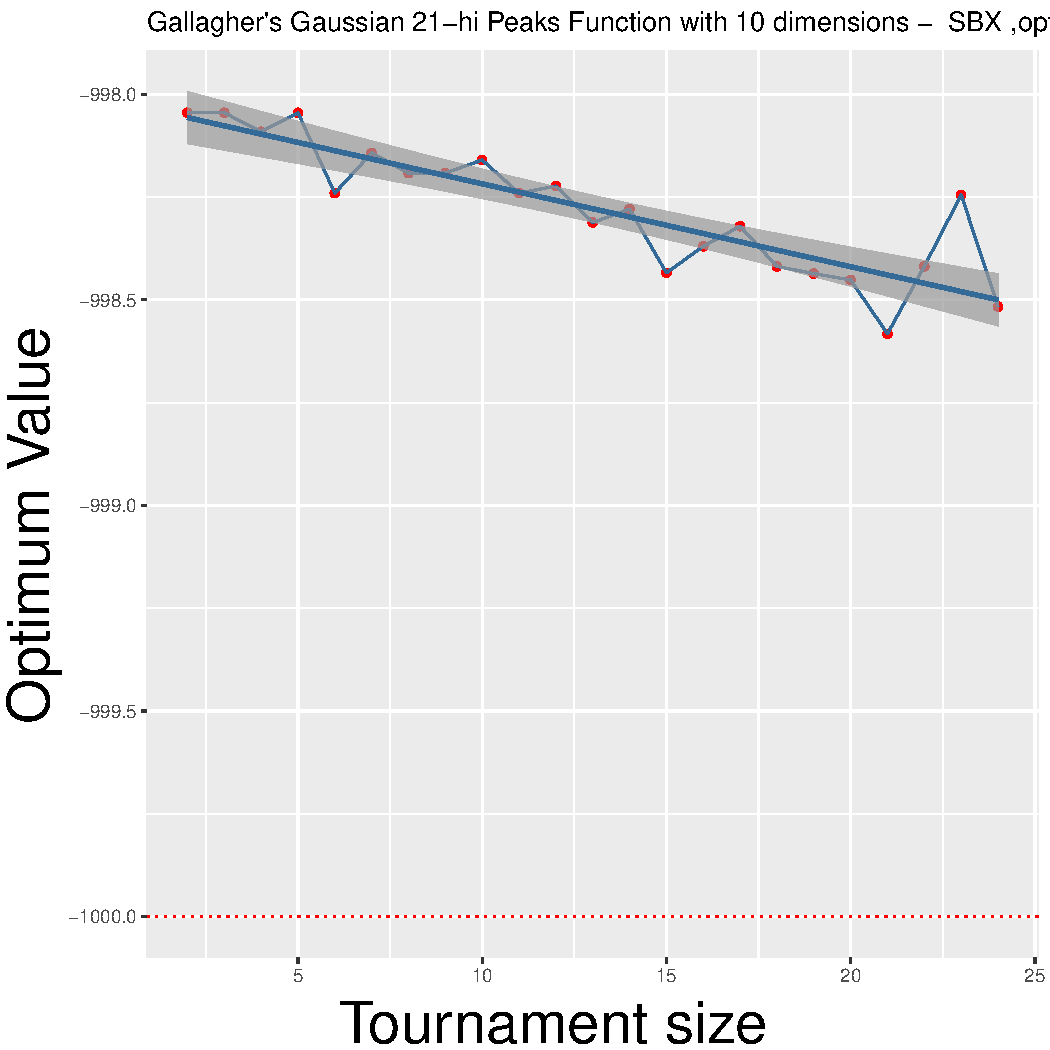
\includegraphics[width=\textwidth]{img/SBX-10D/multimodal_sbx_22_dim_10.pdf}
		\caption{10 dimensions.}
	\end{subfigure}
	\begin{subfigure}[b]{0.33\textwidth}
		\centering
			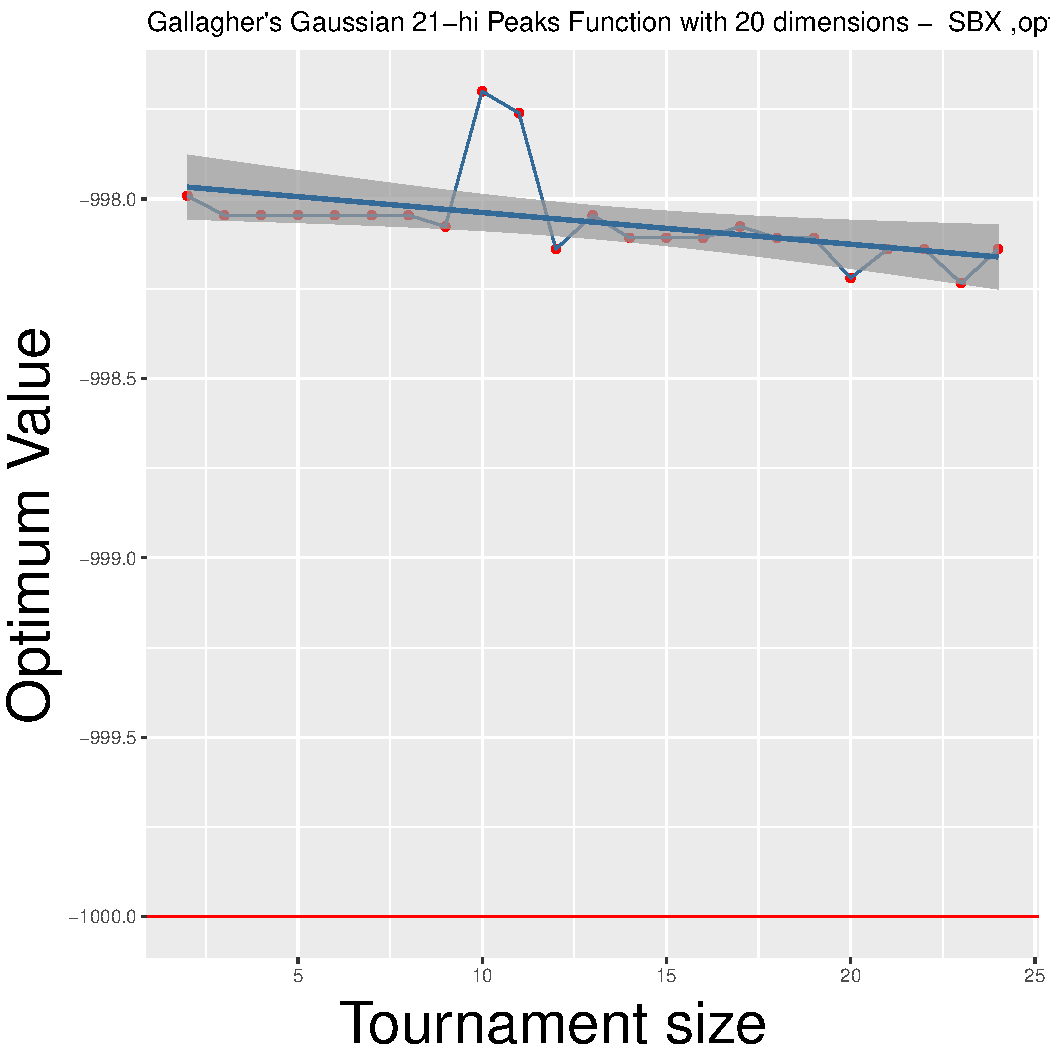
\includegraphics[width=\textwidth]{img/SBX-20D/multimodal_sbx_22_dim_20.pdf}
		\caption{20 dimensions.}
	\end{subfigure}
	\begin{subfigure}[b]{0.33\textwidth}
		\centering
		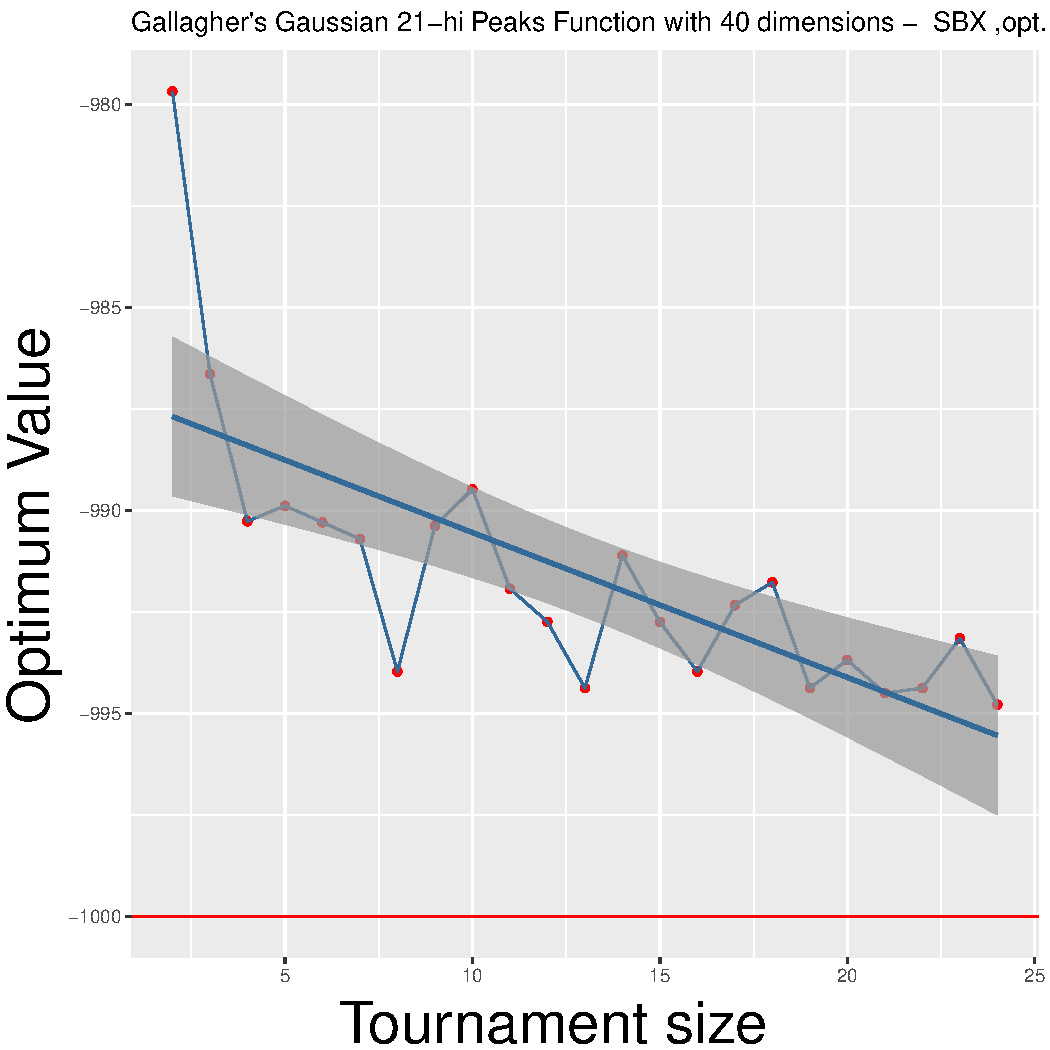
\includegraphics[width=\textwidth]{img/SBX-40D/multimodal_sbx_22_dim_40.pdf}
		\caption{40 dimensions.}
	\end{subfigure}
	\caption{Average performance on different tournament size for the Gallagher's Gaussian 21-hi Peaks Function, when using the SBX crossover - ($\lambda, \lambda$) scheme.}
	\label{sbx-22}
\end{figure*}

\begin{figure*}[t]
	\begin{subfigure}[b]{0.33\textwidth}
		\centering
		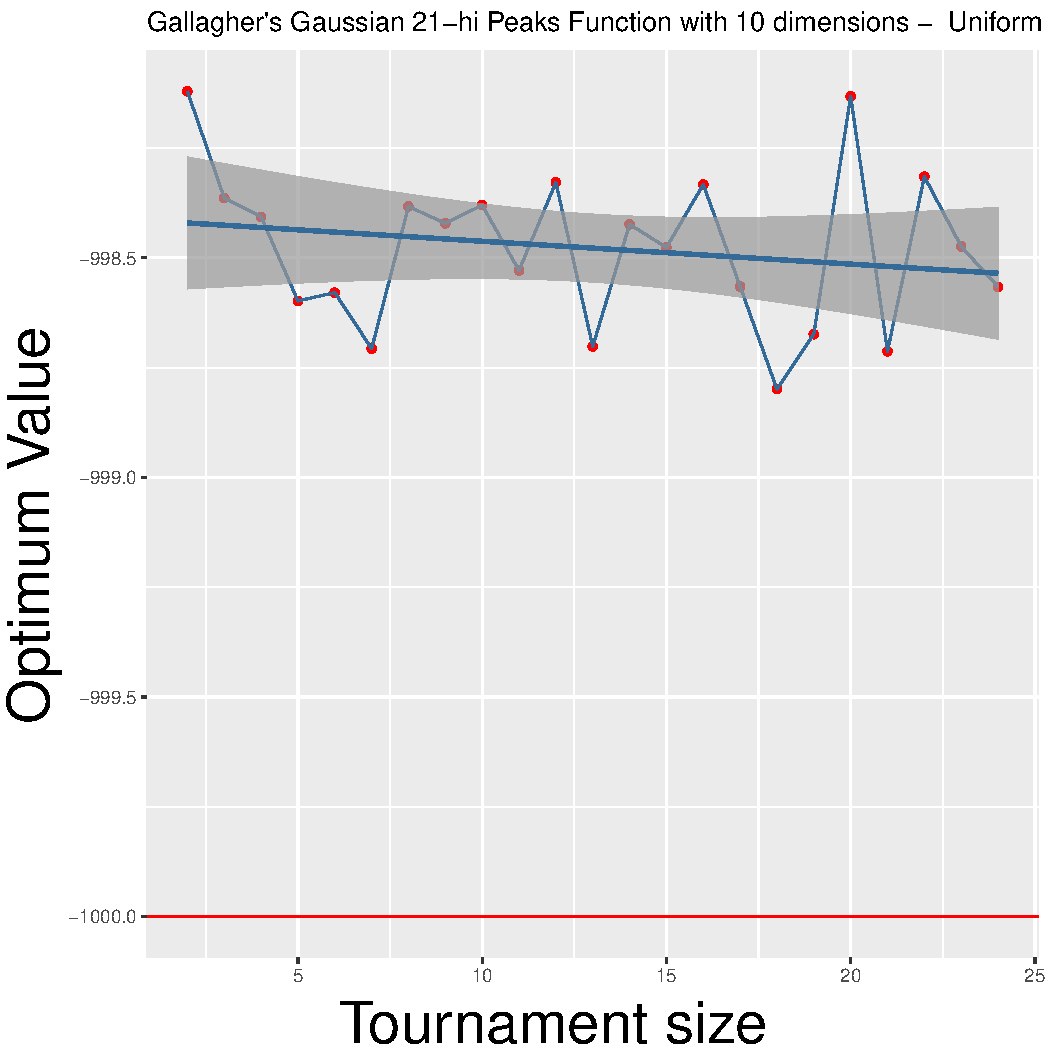
\includegraphics[width=\textwidth]{img/uniform-10D/multimodal_uniform_22_dim_10.pdf}
		\caption{10 dimensions.}
	\end{subfigure}
	\begin{subfigure}[b]{0.33\textwidth}
		\centering
		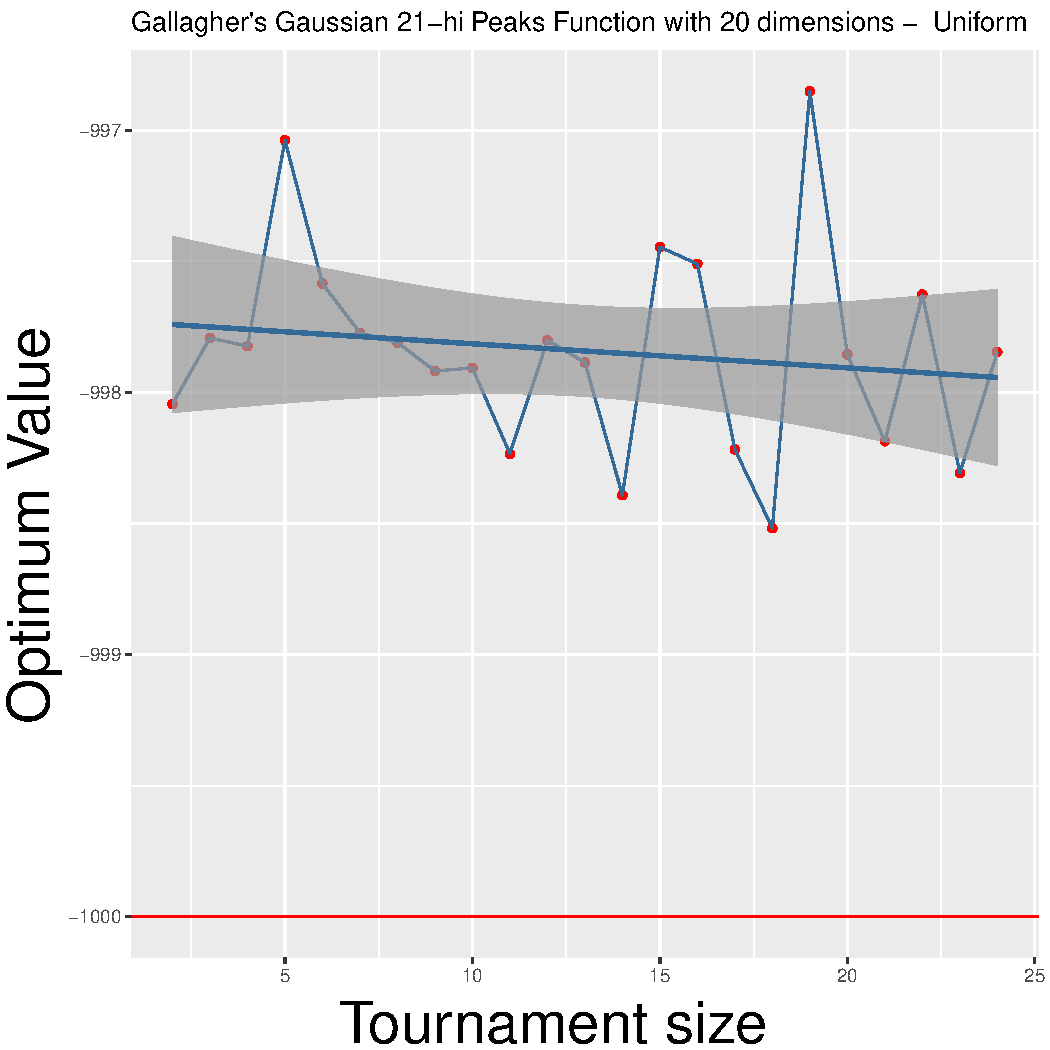
\includegraphics[width=\textwidth]{img/uniform-20D/multimodal_uniform_22_dim_20.pdf}
		\caption{20 dimensions.}
	\end{subfigure}
	\begin{subfigure}[b]{0.33\textwidth}
		\centering
		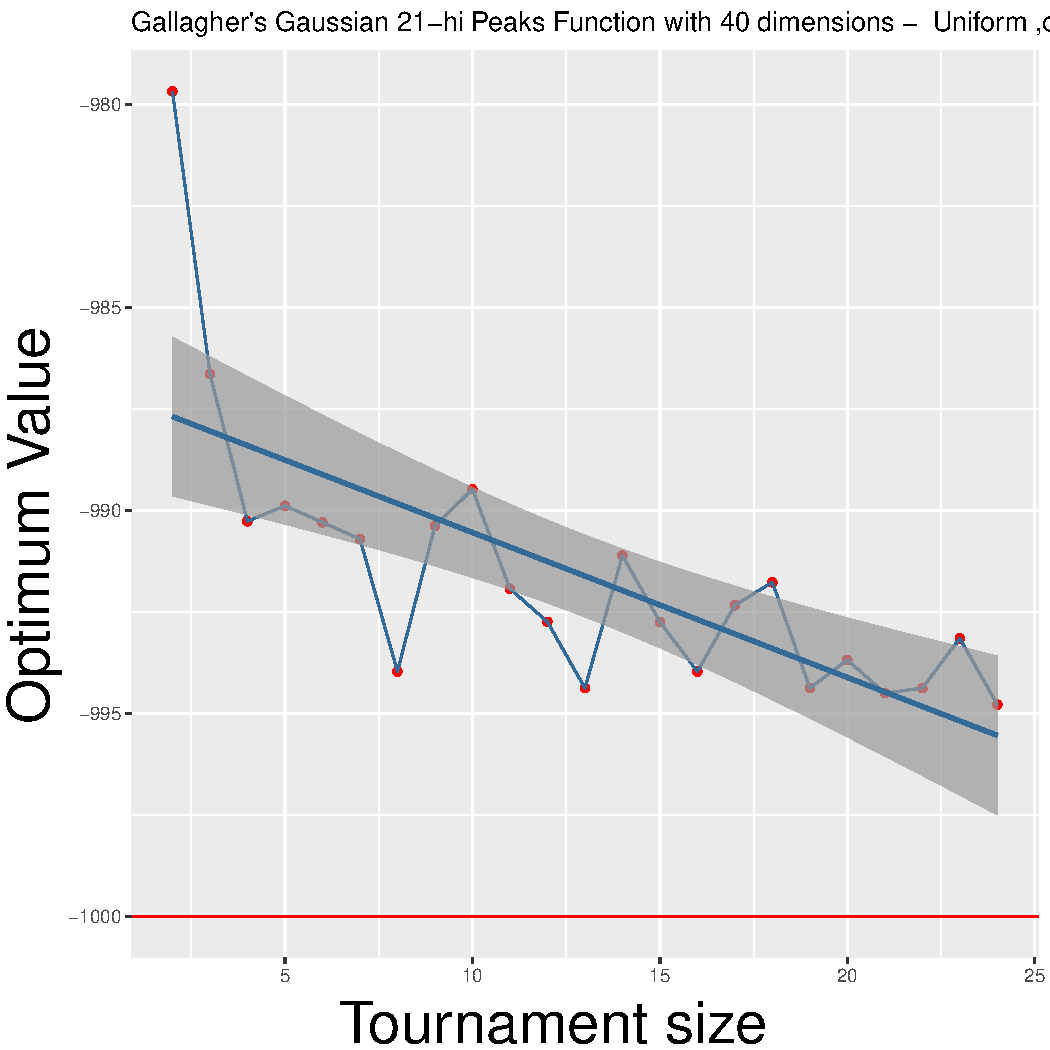
\includegraphics[width=\textwidth]{img/uniform-40D/multimodal_uniform_22_dim_40.pdf}
		\caption{40 dimensions.}
	\end{subfigure}
	\caption{Average performance on different tournament size for the Gallagher's Gaussian 21-hi Peaks Function, when using the uniform crossover - ($\lambda, \lambda$) scheme.}
	\label{uniform-22}
\end{figure*}

\begin{figure*}[t]
	\begin{subfigure}[b]{0.33\textwidth}
		\centering
		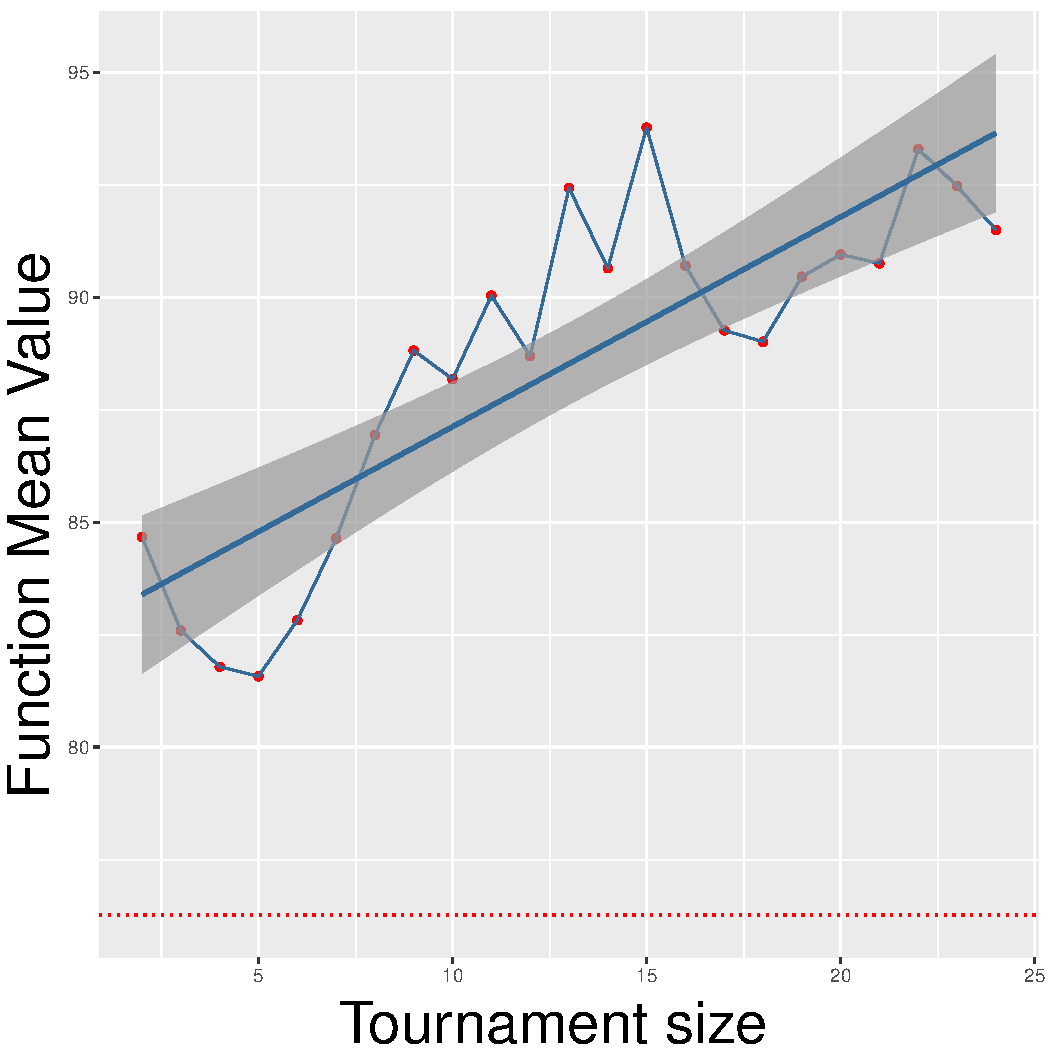
\includegraphics[width=\textwidth]{img/SBX-10D/unimodal_sbx_11_dim_10.pdf}
		\caption{10 dimensions.}
	\end{subfigure}
	\begin{subfigure}[b]{0.33\textwidth}
		\centering
		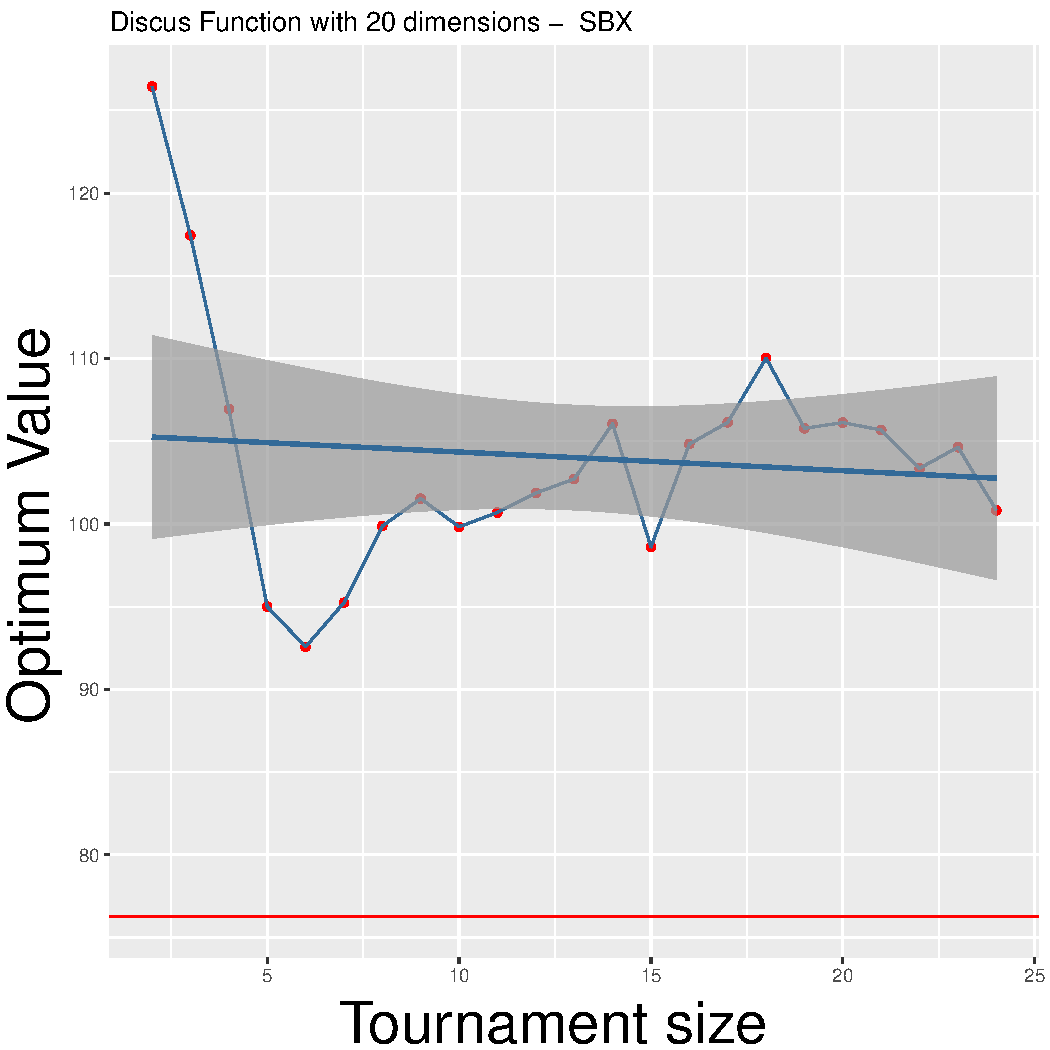
\includegraphics[width=\textwidth]{img/SBX-20D/unimodal_sbx_11_dim_20.pdf}
		\caption{20 dimensions.}
	\end{subfigure}
	\begin{subfigure}[b]{0.33\textwidth}
		\centering
		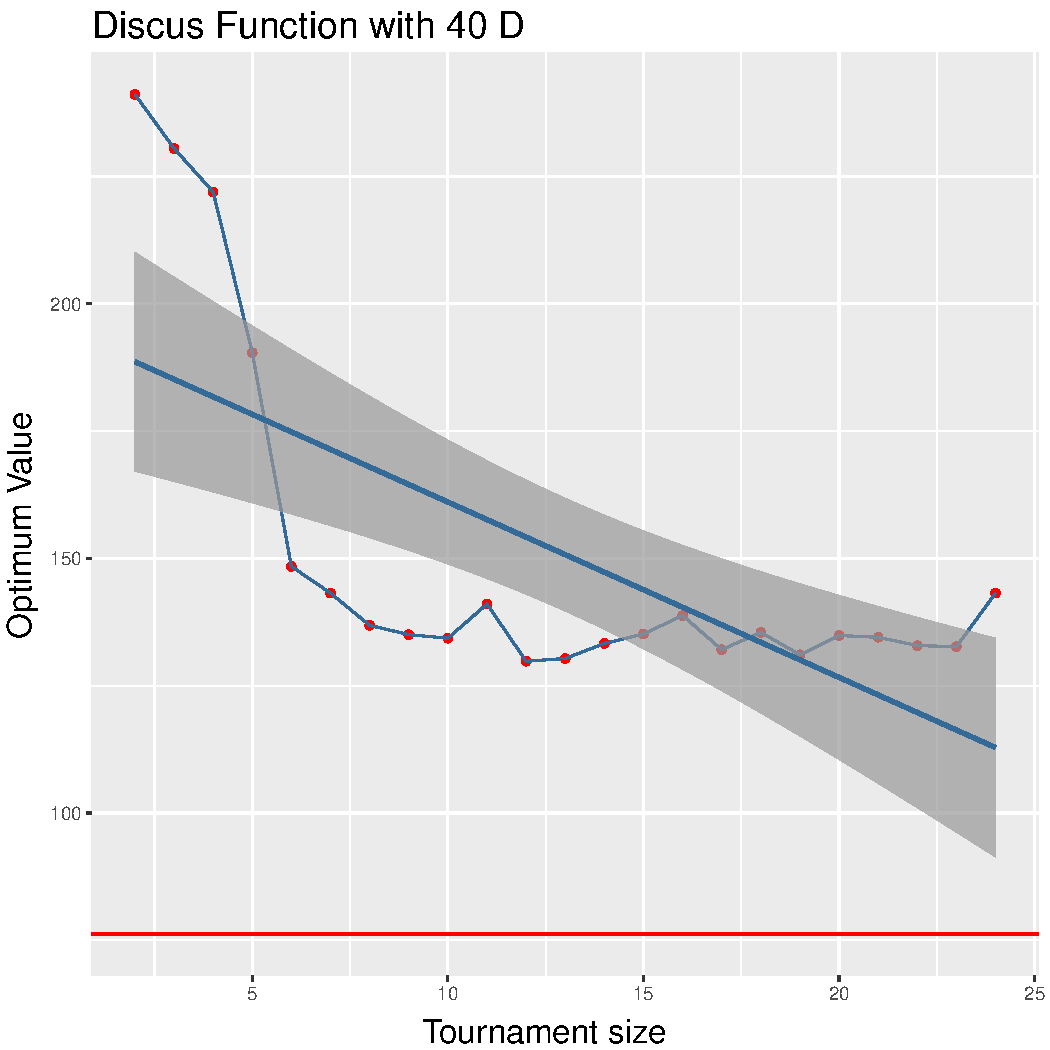
\includegraphics[width=\textwidth]{img/SBX-40D/unimodal_sbx_11_dim_40.pdf}
		\caption{40 dimensions.}
	\end{subfigure}
	\caption{Average performance on different tournament size for the Discus Function, when using the SBX crossover -($\lambda, \lambda$) scheme.}
	\label{sbx-11}
\end{figure*}


\begin{figure*}[t]
	\begin{subfigure}[b]{0.33\textwidth}
		\centering
		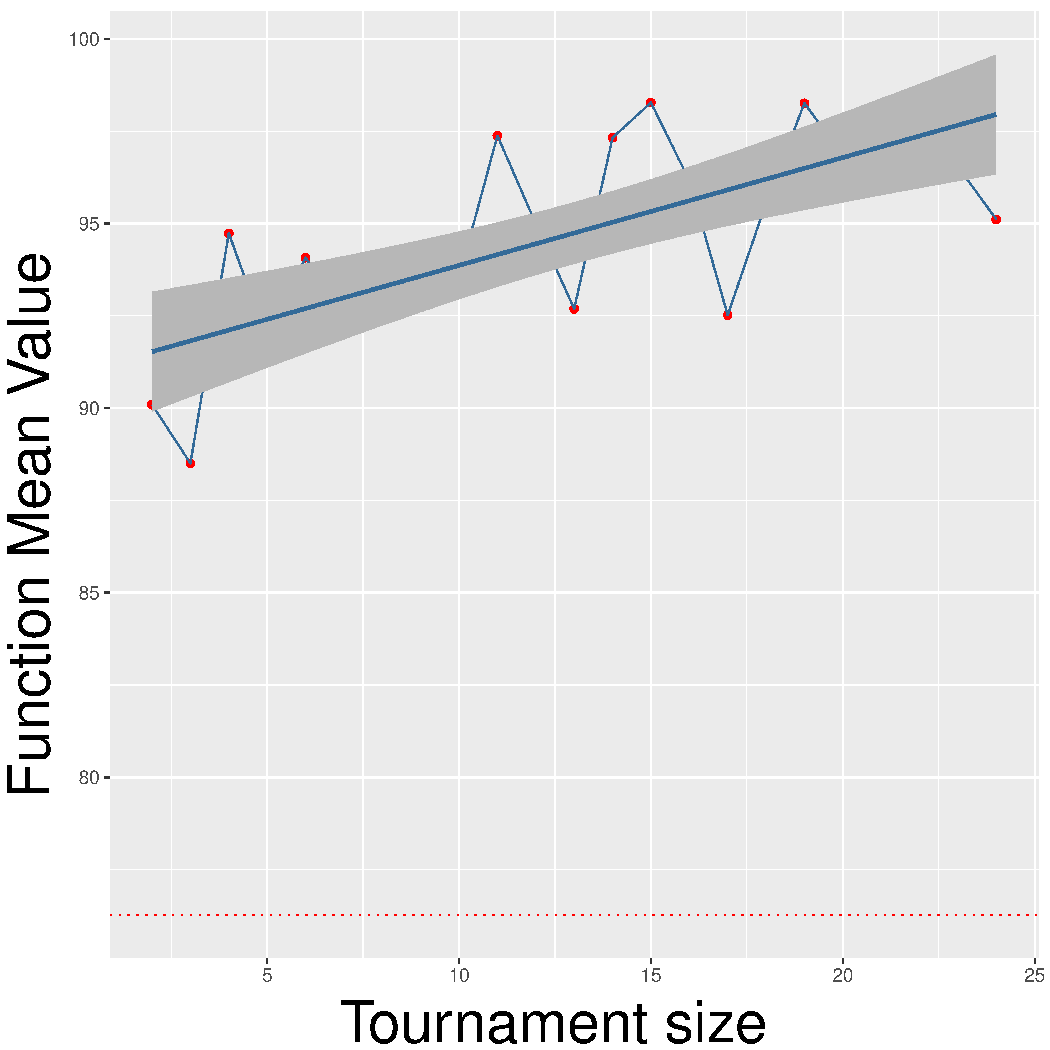
\includegraphics[width=\textwidth]{img/uniform-10D/unimodal_uniform_11_dim_10.pdf}
		\caption{10 dimensions.}
	\end{subfigure}
	\begin{subfigure}[b]{0.33\textwidth}
		\centering
		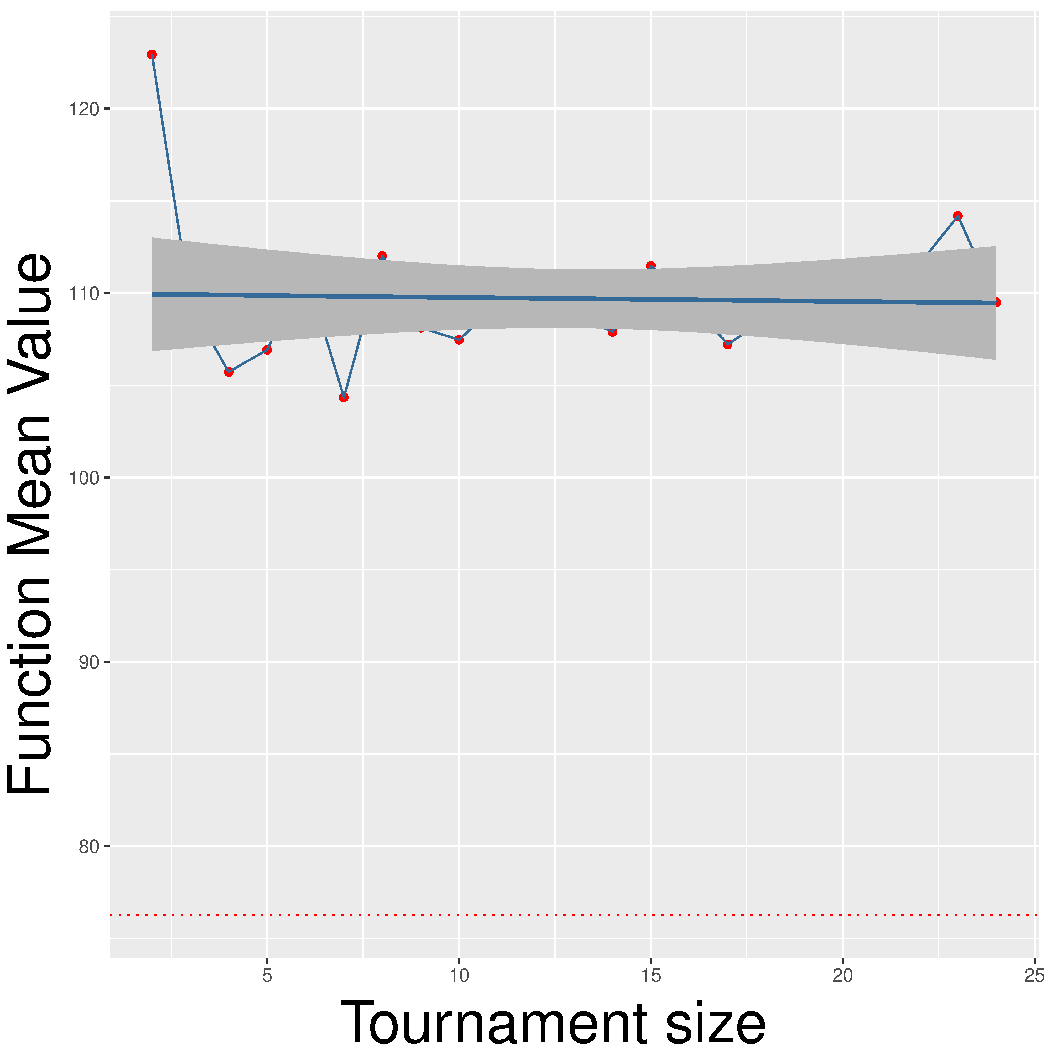
\includegraphics[width=\textwidth]{img/uniform-20D/unimodal_uniform_11_dim_20.pdf}
		\caption{20 dimensions.}
	\end{subfigure}
	\begin{subfigure}[b]{0.33\textwidth}
		\centering
		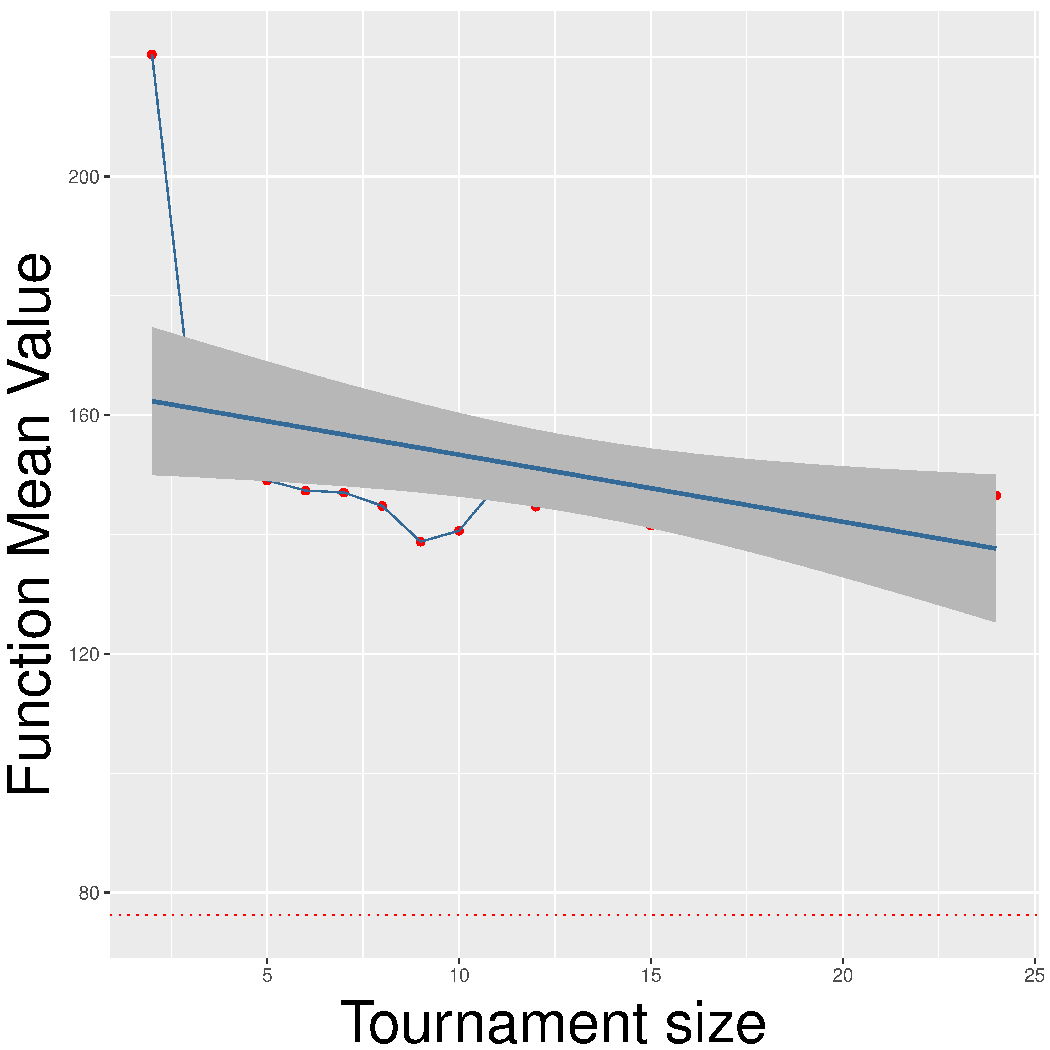
\includegraphics[width=\textwidth]{img/uniform-40D/unimodal_uniform_11_dim_40.pdf}
		\caption{40 dimensions.}
	\end{subfigure}
	\caption{Average performance on different tournament size for the Discus Function, when using the uniform crossover - ($\lambda, \lambda$) scheme.}
	\label{uniform-11}
\end{figure*}


To get a finer intuition about the results, we show  some visual examples, separated in two groups of Figures. The first group, shows the mean value achieved by the GA given a function. The second one, shows the convergence plot with the mean of the values found at each generation, the function target value with a given tournament size. All Figures represent the mean of 40 repetitions given a certain dimension.



\subsection{Tournament Size by Functions Analysis}
The Figures~\ref{sbx-22} and ~\ref{uniform-22} exemplify that for the Gallagher's Gaussian 21-hi Peaks Function (with 10, 20 and 40 dimensions) changing the tournament size for higher values tend to increase the quality of the results, with greater variation when the SBX crossovers, Figure~\ref{sbx-22}, in used when comparing with the uniform crossover. Figure~\ref{uniform-22}.

For the Discus Function, the Figures~\ref{sbx-11},~\ref{uniform-11}, (with 10, 20 and 40 dimensions) show that the same trend is observed. 

The gray shaded area represents the 95\% confidence level interval for predictions from a linear model for each scenario showed and demonstrate that choosing small values for the tournament size, as 2 or 3 can be a very poor choice. For all Figures, the mean of 40 repetitions is shown as bullets and the red line is shows the objective target value for the function.


\subsection{Convergence Analysis}
The Figures~\ref{convegence-11} and~\ref{convergence-23} exemplify that for the Discus Function with 40 dimensions and with the SBX crossover the GA is converging towards the optimum target value, represented by the bottom, red, horizontal line. The same convergence is observed with the uniform crossover for the Katsuura Function. We found similar behavior in most of the functions, given any crossover operator.

\begin{figure}[t]
	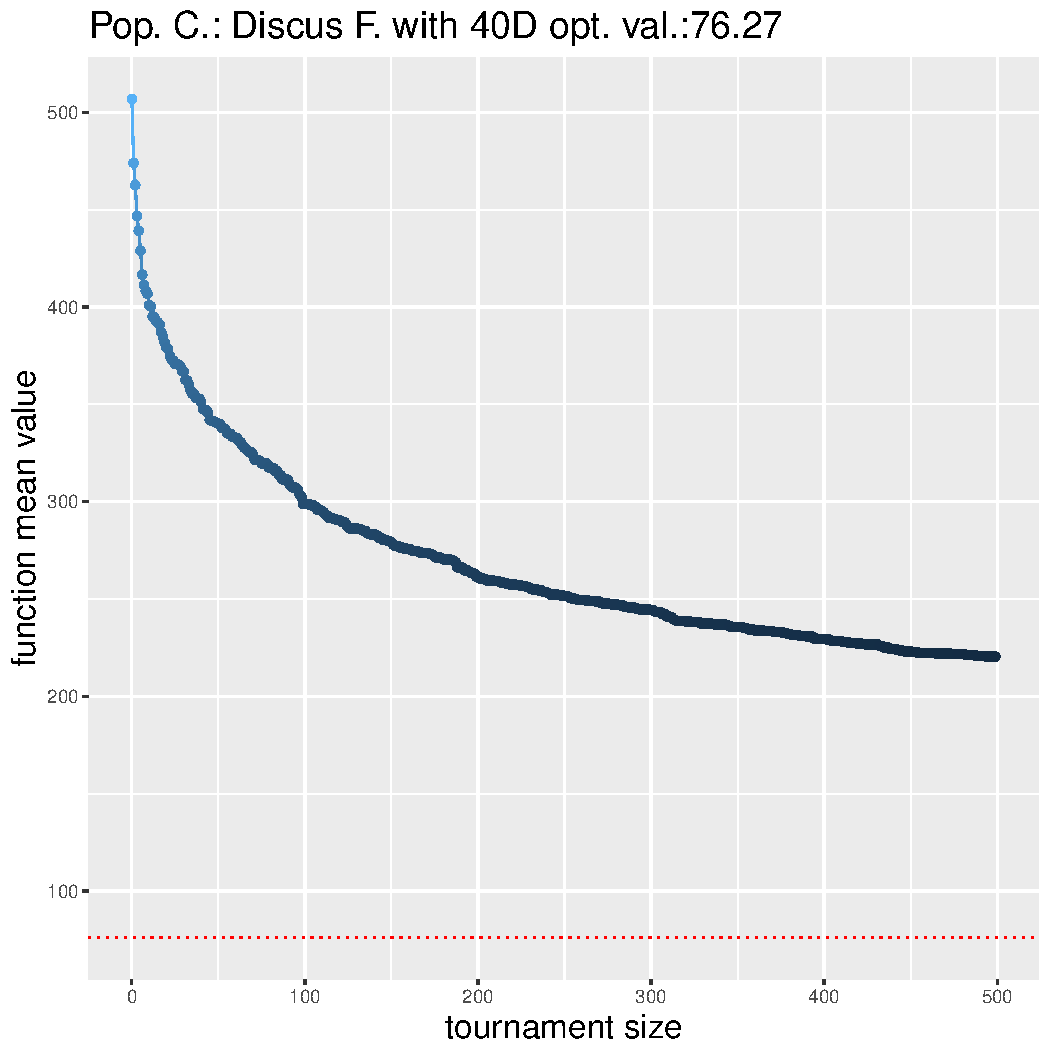
\includegraphics[width=0.5\textwidth]{img/uniform-40D/covergency_unimodal_uniform_11_dim_40.pdf}
	\caption{Population convergence for Discus Function.}
	\label{convegence-uniform-11}
\end{figure}


\begin{figure}[t]
	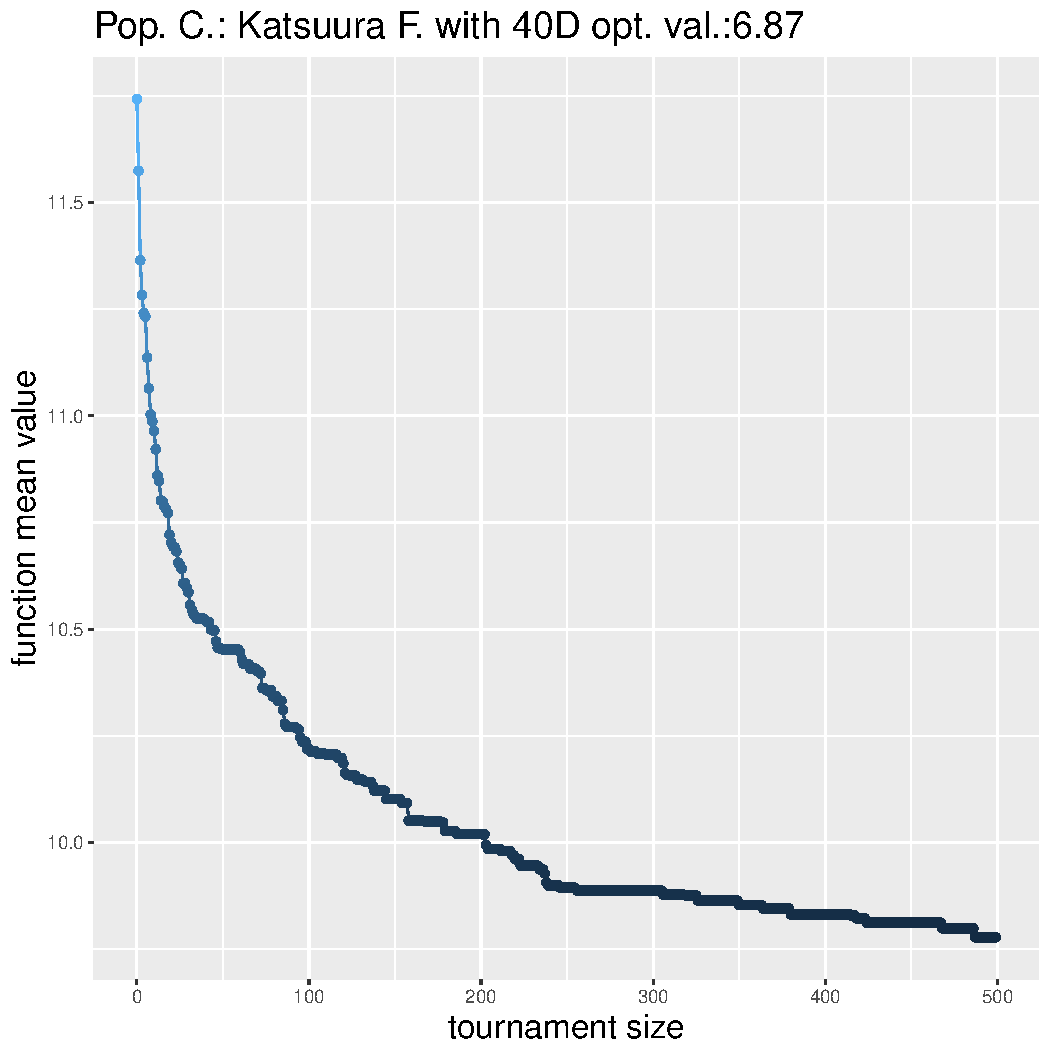
\includegraphics[width=0.5\textwidth]{img/SBX-40D/covergency_multimodal_sbx_23_dim_40.pdf}
	\caption{Population convergence for Katsuura Function.}
	\label{convergence-23}
\end{figure}


\subsection{($\lambda + \lambda$) scheme}


The Friedman Test showed significant difference in values among tournament size values across all functions, for any configuration, with the SBX crossover. This results hold for every scenario with 40 dimensions, given: all functions (unimodal or multimodal); only the unimodal functions; or only the multimodal functions. 

\begin{table}[h]
	\centering
	\begin{tabular}{|l|l|l|l|}
		\hline
		\textbf{Function Group} & \textbf{Dimension size}      & \textbf{Chi-squared}        & \textbf{P-value}                     \\ \hline
		\multicolumn{1}{|l|}{All} & \multicolumn{1}{|l|}{10} & \multicolumn{1}{l|}{118.67} & \multicolumn{1}{l|}{3.035e-15} \\ \hline
		\multicolumn{1}{|l|}{Unimodal} & \multicolumn{1}{|l|}{10} & \multicolumn{1}{l|}{54.011} & \multicolumn{1}{l|}{0.0001639} \\ \hline
		\multicolumn{1}{|l|}{Multimodal} & \multicolumn{1}{|l|}{10} & \multicolumn{1}{l|}{75.724} & \multicolumn{1}{l|}{8.073e-08}  \\ \hline
		\hline
		\multicolumn{1}{|l|}{All} & \multicolumn{1}{|l|}{20} & \multicolumn{1}{l|}{157.29} & \multicolumn{1}{l|}{< 2.2e-16} \\ \hline
		\multicolumn{1}{|l|}{Unimodal} & \multicolumn{1}{|l|}{20} & \multicolumn{1}{l|}{73.078} & \multicolumn{1}{l|}{2.15e-07} \\ \hline
		\multicolumn{1}{|l|}{Multimodal} & \multicolumn{1}{|l|}{20} & \multicolumn{1}{l|}{95.524} & \multicolumn{1}{l|}{3.867e-11}  \\ \hline
		\hline	
		\multicolumn{1}{|l|}{All} & \multicolumn{1}{|l|}{40} & \multicolumn{1}{l|}{190.59} & \multicolumn{1}{l|}{< 2.2e-16} 						\\ \hline
		\multicolumn{1}{|l|}{Unimodal} & \multicolumn{1}{|l|}{40} & \multicolumn{1}{l|}{101.52} & \multicolumn{1}{l|}{3.502e-12} \\ \hline
		\multicolumn{1}{|l|}{Multimodal} & \multicolumn{1}{|l|}{40} & \multicolumn{1}{l|}{87.318} & \multicolumn{1}{l|}{9.762e-10}  \\ \hline
	\end{tabular}
	\caption{Friedman Test results for SBX Crossover - ($\lambda + \lambda$) scheme.}
	\label{Friedman_test_uniform-B}	
\end{table}

As for the generation ($\lambda, \lambda$), we show visual examples to get a finer intuition about the results, we show  some visual examples, separated in two groups of Figures. The first group, shows the mean value achieved by the GA given a function. The second one, shows the convergence plot with the mean of the values found at each generation, the function target value with a given tournament size. All Figures represent the mean of 30 repetitions given a certain dimension.


\begin{figure*}[t]
	\begin{subfigure}[b]{0.33\textwidth}
		\centering
		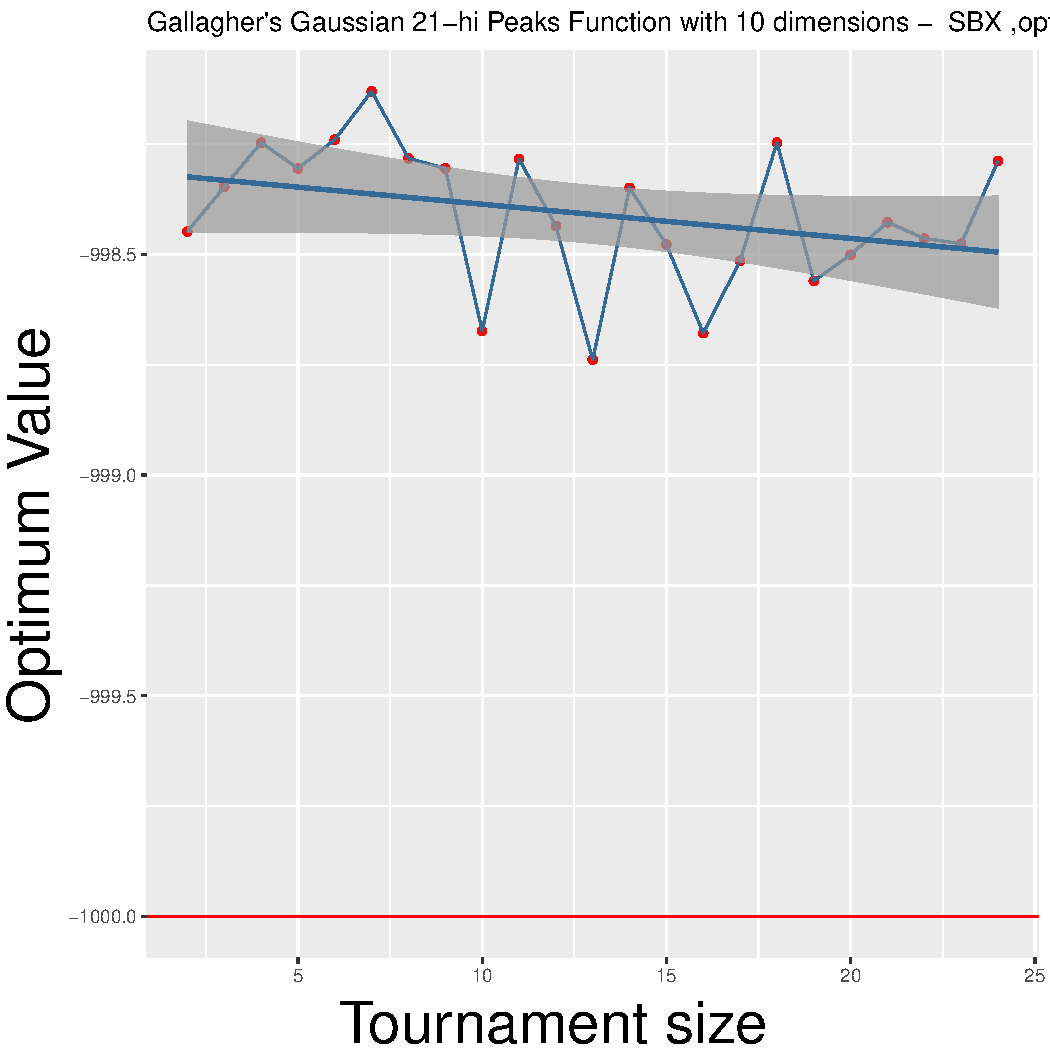
\includegraphics[width=\textwidth]{img/2n2n-10D/multimodal_2n2n_22_dim_10.pdf}
		\caption{10 dimensions.}
	\end{subfigure}
	\begin{subfigure}[b]{0.33\textwidth}
		\centering
		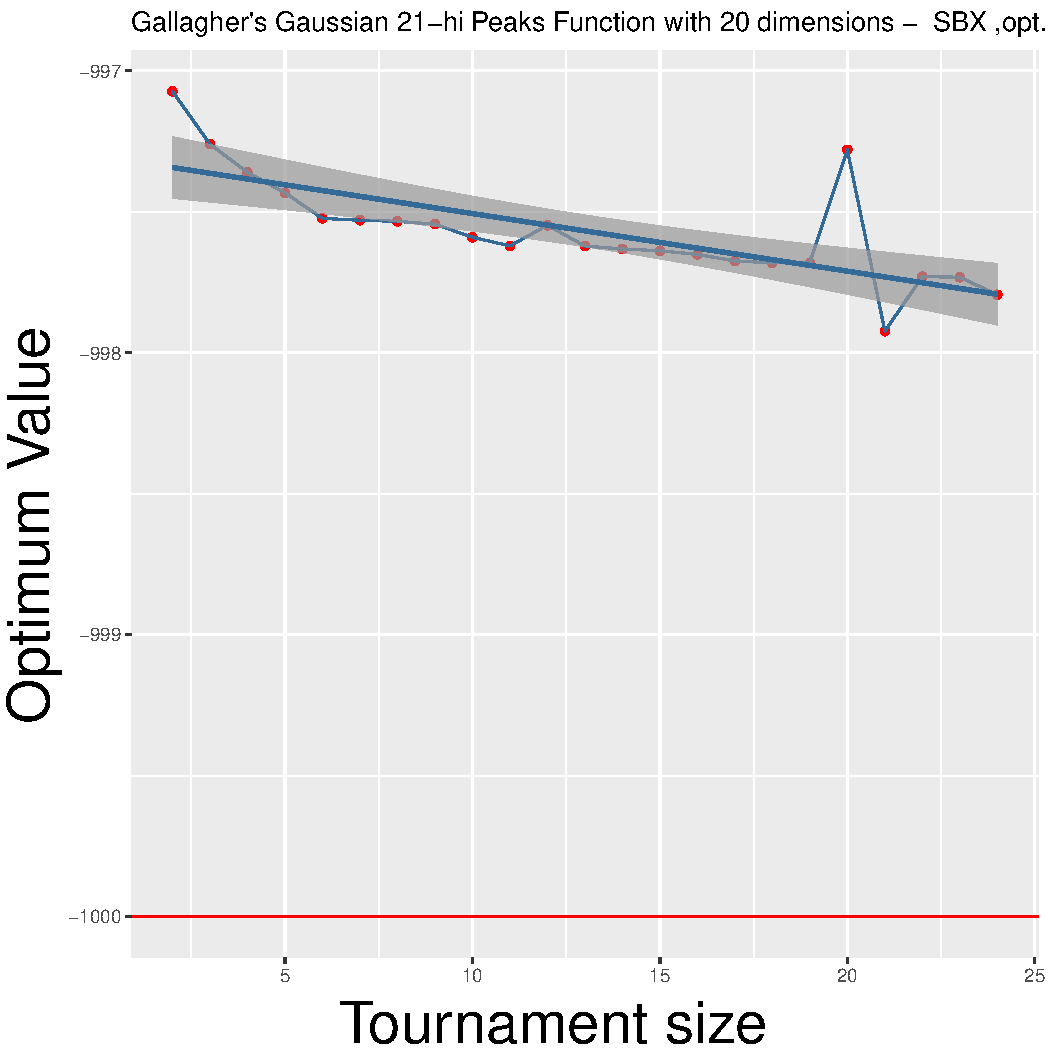
\includegraphics[width=\textwidth]{img/2n2n-20D/multimodal_2n2n_22_dim_20.pdf}
		\caption{20 dimensions.}
	\end{subfigure}
	\begin{subfigure}[b]{0.33\textwidth}
		\centering
		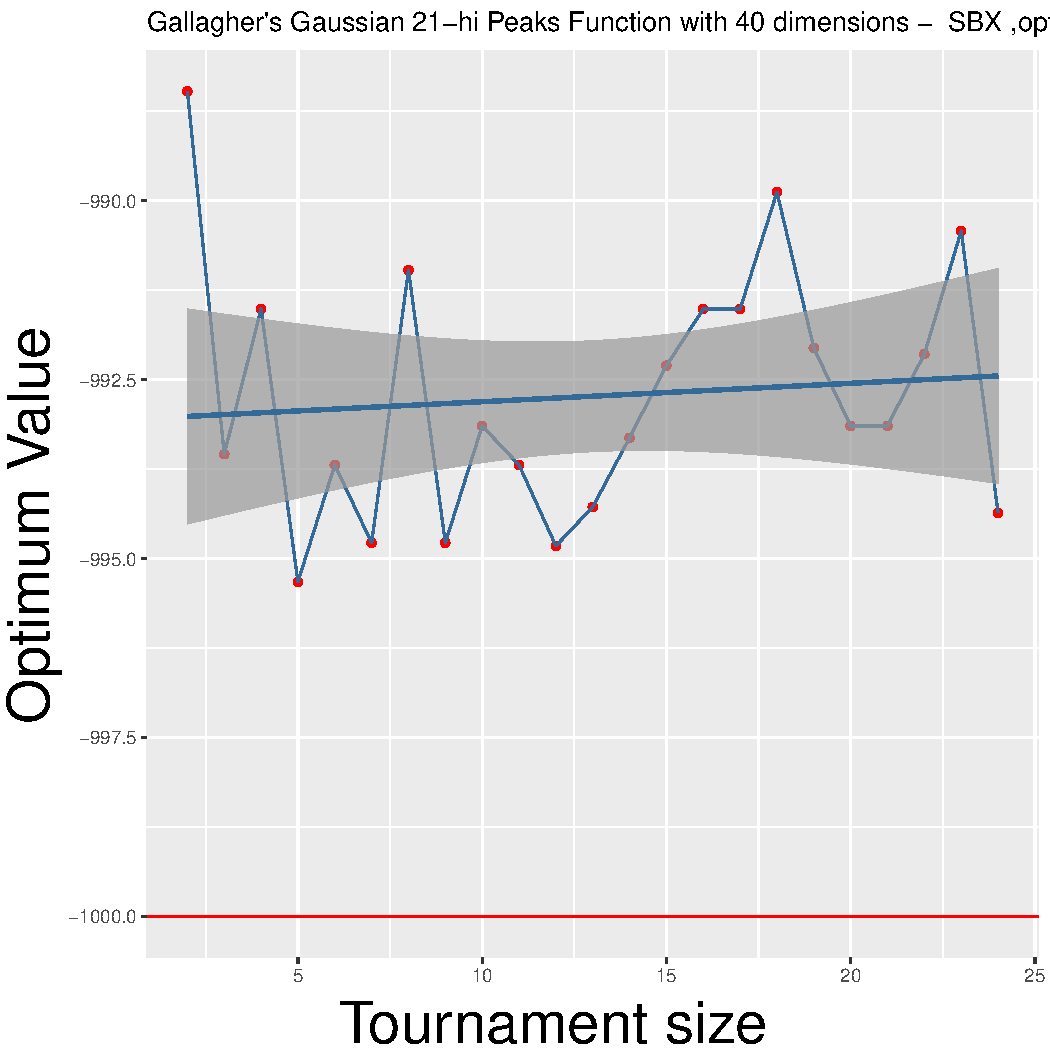
\includegraphics[width=\textwidth]{img/2n2n-40D/multimodal_2n2n_22_dim_40.pdf}
		\caption{40 dimensions.}
	\end{subfigure}
	\caption{Average performance on different tournament size for the Gallagher's Gaussian 21-hi Peaks Function, when using the SBX crossover - ($\lambda + \lambda$) scheme.}
	\label{sbx-22-B}
\end{figure*}

\begin{figure*}[t]
	\begin{subfigure}[b]{0.33\textwidth}
		\centering
		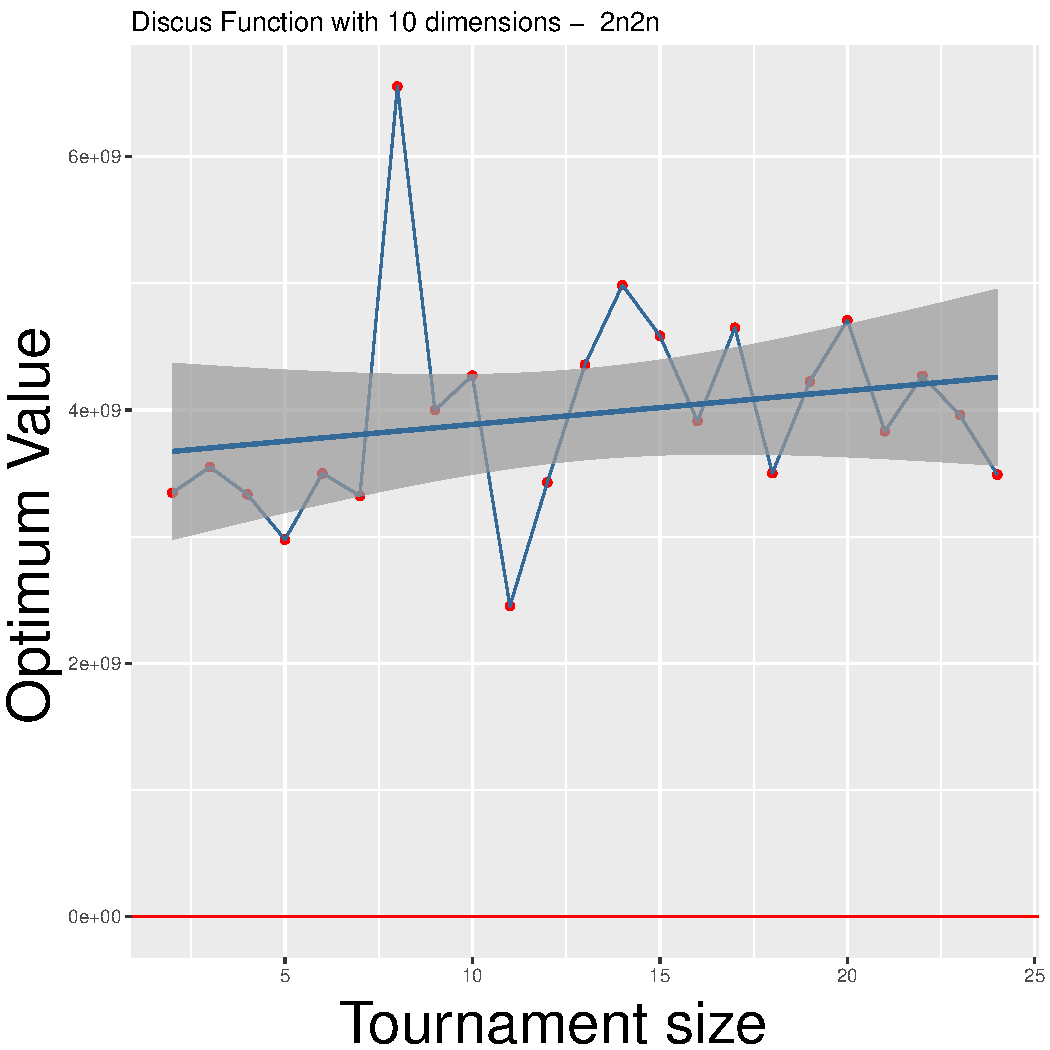
\includegraphics[width=\textwidth]{img/2n2n-10D/unimodal_2n2n_11_dim_10.pdf}
		\caption{10 dimensions.}
	\end{subfigure}
	\begin{subfigure}[b]{0.33\textwidth}
		\centering
		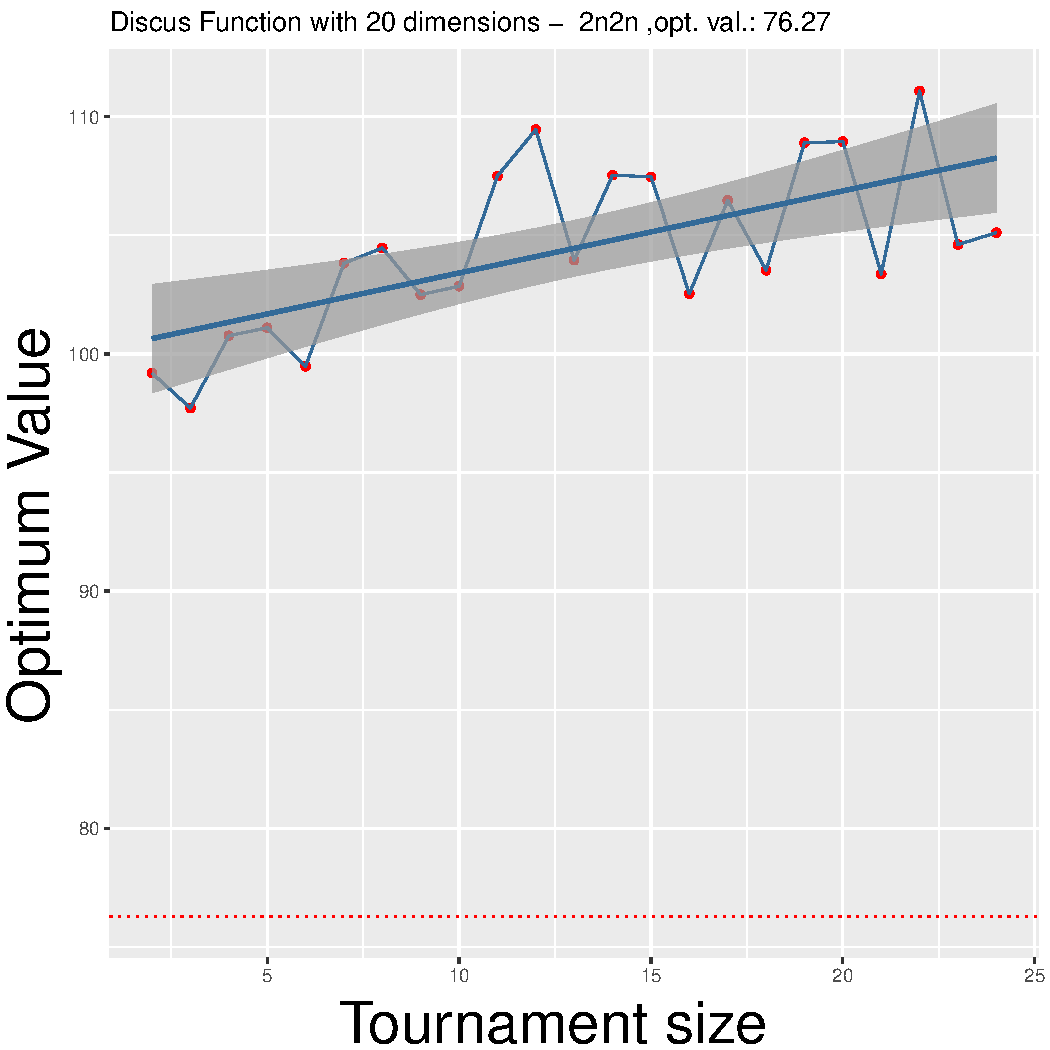
\includegraphics[width=\textwidth]{img/2n2n-20D/unimodal_2n2n_11_dim_20.pdf}
		\caption{20 dimensions.}
	\end{subfigure}
	\begin{subfigure}[b]{0.33\textwidth}
		\centering
		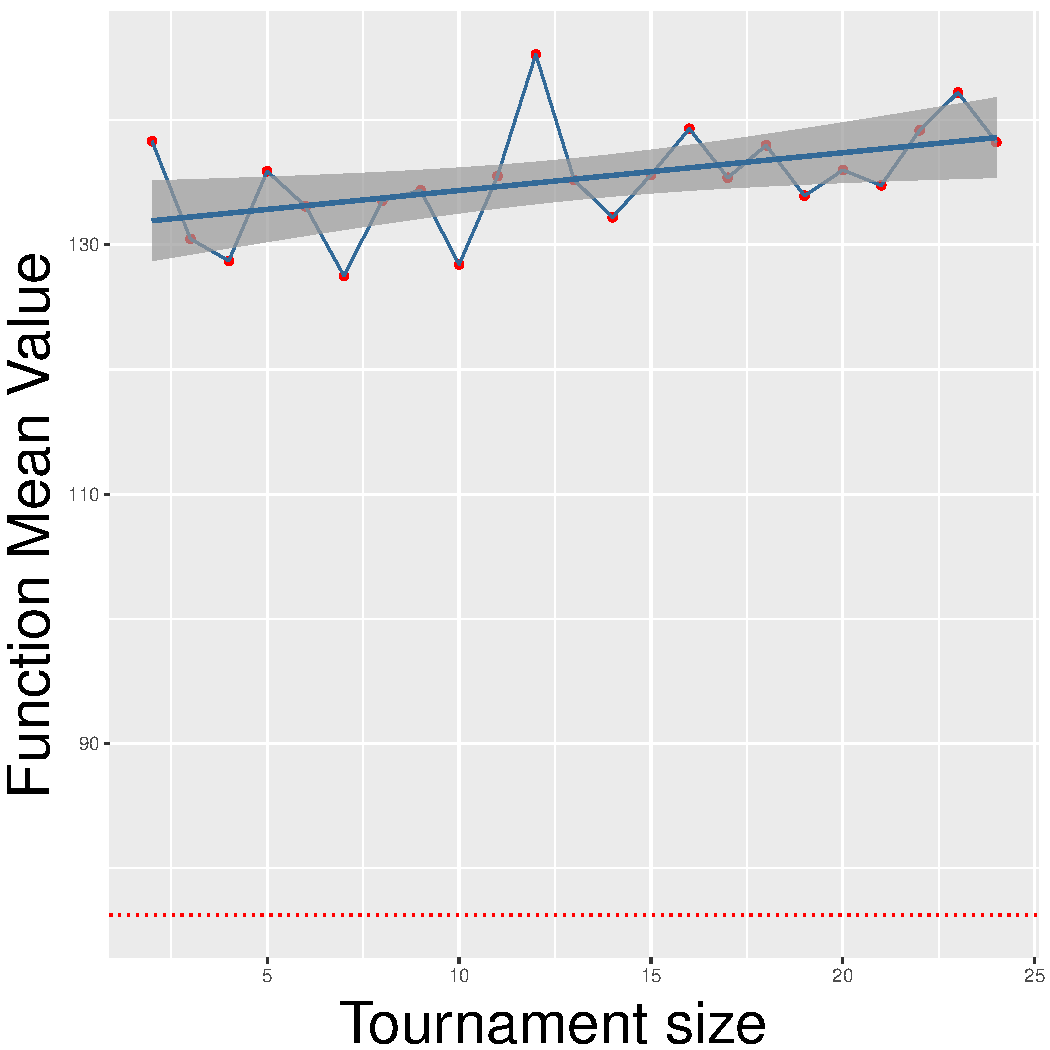
\includegraphics[width=\textwidth]{img/2n2n-40D/unimodal_2n2n_11_dim_40.pdf}
		\caption{40 dimensions.}
	\end{subfigure}
	\caption{Average performance on different tournament size for the Discus Function, when using the SBX crossover - ($\lambda + \lambda$) scheme.}
	\label{sbx-11-B}
\end{figure*}


\subsection{Tournament Size by Functions Analysis}
The Figure~\ref{sbx-22-B} that exemplifies that for the Gallagher's Gaussian 21-hi Peaks Function (with 10, 20 and 40 dimensions) changing the tournament size does not lead to significant better final values found by the GA. The Figure~\ref{sbx-11-B} shows the same trend, but for the Discus Function.

The gray shaded area represents the 95\% confidence level interval for predictions from a linear model for each scenario showed and demonstrate that choosing small values for the tournament size, as 2 or 3 can be a very poor choice. For all Figures, the mean of 30 repetitions is shown as bullets and the red line is shows the objective target value for the function.


\subsection{Convergence Analysis}
The Figures~\ref{convegence-11} and~\ref{convergence-23} exemplify that for the Discus Function with 40 dimensions and with the SBX crossover the GA is converging towards the optimum target value, represented by the bottom, red, horizontal line. The same convergence is observed with the uniform crossover for the Katsuura Function. We found similar behavior in most of the functions, given any crossover operator.

\begin{figure}[t]
	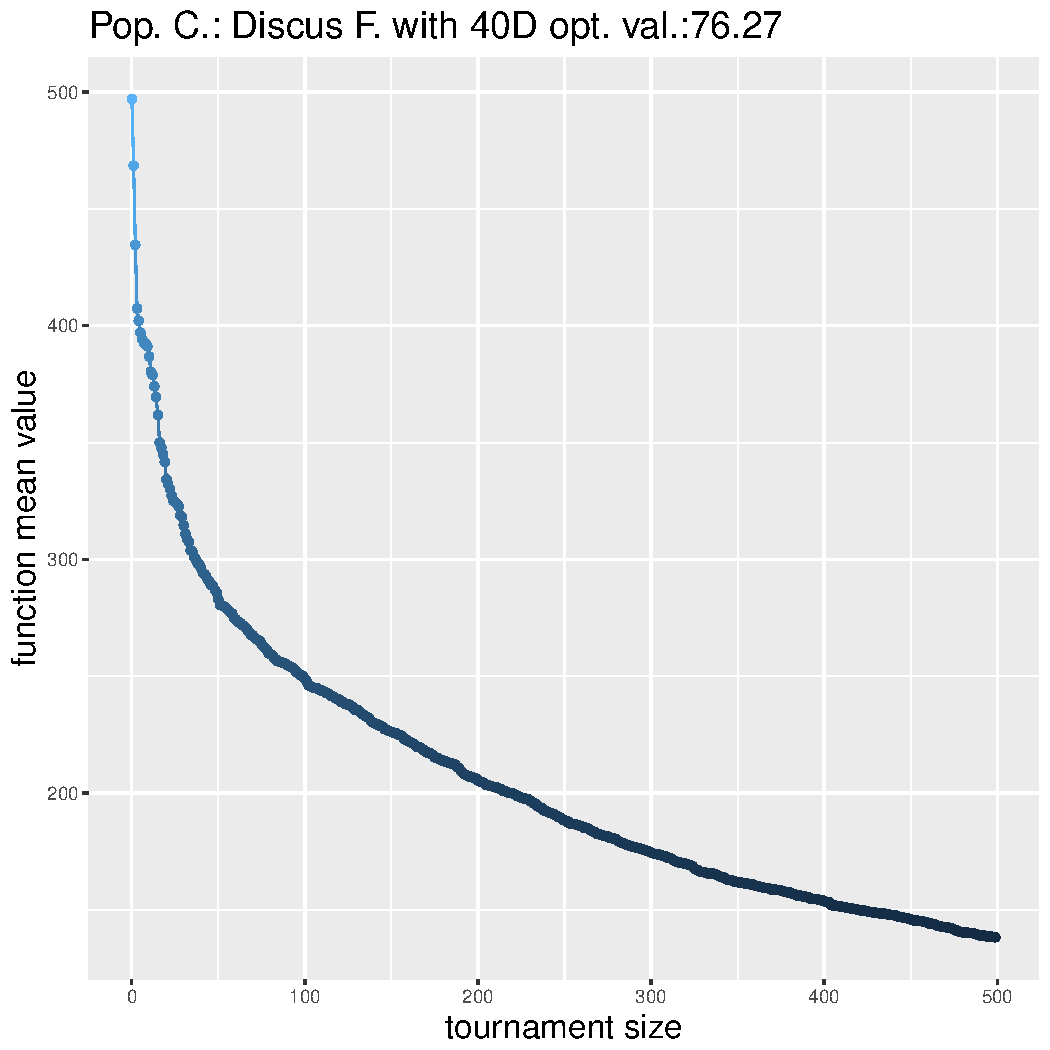
\includegraphics[width=0.5\textwidth]{img/2n2n-40D/covergency_unimodal_2n2n_11_dim_40.pdf}
	\caption{Population convergence for Discus Function.}
	\label{convegence-11}
\end{figure}
